\documentclass[a4paper,12pt]{paper}

\usepackage{mycommands}

% Worked-example layout: boxed problem statement followed by a solution.
\newcounter{example}
\renewenvironment{example}[1]{%  % the paper class already defines "example"
  \refstepcounter{example}%
  \begin{mdframed}[linewidth=1pt,innertopmargin=6pt,innerbottommargin=6pt]%
  \noindent\textbf{Example \theexample: #1.}\ }{%
  \end{mdframed}}
\newenvironment{solution}{\par\noindent\textbf{Solution.}\ }{\par\medskip}

\title{Worked examples for Lecture 19: Waveform tomography}
\author{David Al-Attar \\ Michaelmas Term, \the\year}

\begin{document}

\maketitle

\noindent These examples accompany Lecture~19. They are intended as practice in the concrete
calculations that underlie the lecture, and are less demanding than the questions on the
problem sets. The first two apply the Lagrange multiplier method to systems small enough that every
step can be written out, the third looks at the convergence of steepest descent, the fourth derives the
adjoint traction for a cross-correlation delay time, and the last puts numbers to the cost of the adjoint
method. Numerical results were checked with the scripts in the \texttt{python} directory.

%-----------------------------------------------------------------------------------------------
\begin{example}{The adjoint method for a linear system}
Let $\mathbf{A}(\mathbf{m})$ be an invertible $n\times n$ matrix depending smoothly on parameters
$\mathbf{m}=(m_{1},\dots,m_{m})$, let $\mathbf{f}$ be a fixed vector, and define $\mathbf{u}(\mathbf{m})$ by
$\mathbf{A}(\mathbf{m})\mathbf{u}=\mathbf{f}$. Data are predicted by $\mathbf{P}\mathbf{u}$, with $\mathbf{P}$ a fixed
$p\times n$ matrix, and the misfit is $J=\frac{1}{2}\|\mathbf{P}\mathbf{u}-\mathbf{d}\|^{2}$ for observed
data $\mathbf{d}$. Obtain $\partial J/\partial m_{k}$ (i) by direct differentiation and (ii) using the Lagrangian
$L(\mathbf{u},\mathbf{u}',\mathbf{m})=J(\mathbf{u})-\mathbf{u}'^{T}[\mathbf{A}(\mathbf{m})\mathbf{u}-\mathbf{f}]$.
Count the number of linear solves each approach requires, and check the result on
$\mathbf{A}(m)=\begin{pmatrix}2&-1\\-1&m\end{pmatrix}$, $\mathbf{f}=(1,0)^{T}$, $\mathbf{P}=(0\;\;1)$, $d=\frac{1}{2}$ at $m=1$.
\end{example}

\begin{solution}
This is the finite-dimensional skeleton of the calculation in the lecture: the matrix $\mathbf{A}(\mathbf{m})$ stands for
the wave operator, $\mathbf{u}$ for the wavefield, $\mathbf{P}$ for the operation of recording the wavefield at the seismometer,
and $\mathbf{u}'$ for the adjoint wavefield. Because the constraint is a single algebraic equation there is no need for a second
multiplier playing the role of $\mathbf{w}'$.

\emph{Direct differentiation.} Write $\mathbf{r}=\mathbf{P}\mathbf{u}-\mathbf{d}$ for the residual, so that
$J=\frac{1}{2}\mathbf{r}^{T}\mathbf{r}$ and, by the chain rule,
\begin{equation}
\frac{\partial J}{\partial m_{k}}=\mathbf{r}^{T}\mathbf{P}\frac{\partial\mathbf{u}}{\partial m_{k}}.
\label{eq:1}
\end{equation}
Differentiating $\mathbf{A}\mathbf{u}=\mathbf{f}$ with respect to $m_{k}$ gives
$\frac{\partial\mathbf{A}}{\partial m_{k}}\mathbf{u}+\mathbf{A}\frac{\partial\mathbf{u}}{\partial m_{k}}=\mathbf{0}$, and hence
\begin{equation}
\frac{\partial\mathbf{u}}{\partial m_{k}}=-\mathbf{A}^{-1}\frac{\partial\mathbf{A}}{\partial m_{k}}\mathbf{u},\qquad
\frac{\partial J}{\partial m_{k}}=-\mathbf{r}^{T}\mathbf{P}\mathbf{A}^{-1}\frac{\partial\mathbf{A}}{\partial m_{k}}\mathbf{u}.
\label{eq:2}
\end{equation}
To evaluate this we solve $\mathbf{A}\mathbf{u}=\mathbf{f}$ once, and then for each $k$ solve
$\mathbf{A}\,\partial_{k}\mathbf{u}=-(\partial_{k}\mathbf{A})\mathbf{u}$: a total of $m+1$ linear solves with $\mathbf{A}$.
This is precisely the cost of the finite-difference approach discussed in the lecture, of which the above is the exact limit.

\emph{Lagrangian.} The Lagrangian is
\begin{equation}
L(\mathbf{u},\mathbf{u}',\mathbf{m})=\frac{1}{2}(\mathbf{P}\mathbf{u}-\mathbf{d})^{T}(\mathbf{P}\mathbf{u}-\mathbf{d})
-\mathbf{u}'^{T}[\mathbf{A}(\mathbf{m})\mathbf{u}-\mathbf{f}],
\label{eq:3}
\end{equation}
in which $\mathbf{u}$, $\mathbf{u}'$ and $\mathbf{m}$ are treated as independent. The Lagrange multiplier theorem states that
$\partial J/\partial m_{k}=\partial L/\partial m_{k}$ provided the partial derivatives of $L$ with respect to $\mathbf{u}$
and $\mathbf{u}'$ both vanish. Stationarity with respect to $\mathbf{u}'$ recovers the forward problem
$\mathbf{A}\mathbf{u}=\mathbf{f}$. Stationarity with respect to $\mathbf{u}$ requires, for every $\delta\mathbf{u}$,
\begin{equation}
(\mathbf{P}\mathbf{u}-\mathbf{d})^{T}\mathbf{P}\,\delta\mathbf{u}-\mathbf{u}'^{T}\mathbf{A}\,\delta\mathbf{u}=
\left[\mathbf{P}^{T}(\mathbf{P}\mathbf{u}-\mathbf{d})-\mathbf{A}^{T}\mathbf{u}'\right]^{T}\delta\mathbf{u}=0,
\label{eq:4}
\end{equation}
and hence $\mathbf{u}'$ satisfies the \emph{adjoint equation}
\begin{equation}
\mathbf{A}^{T}\mathbf{u}'=\mathbf{P}^{T}(\mathbf{P}\mathbf{u}-\mathbf{d}).
\label{eq:5}
\end{equation}
The right-hand side is the residual mapped back into the state space by $\mathbf{P}^{T}$; it is the analogue of the
adjoint traction $h_{i}'$ in the lecture, which places the residual seismogram at the receiver location using a delta function.
With both conditions satisfied, the model dependence of $L$ is confined to the matrix $\mathbf{A}(\mathbf{m})$, and so
\begin{equation}
\frac{\partial J}{\partial m_{k}}=\frac{\partial L}{\partial m_{k}}=-\mathbf{u}'^{T}\frac{\partial\mathbf{A}}{\partial m_{k}}\mathbf{u}.
\label{eq:6}
\end{equation}
This agrees with eq.~(\ref{eq:2}), since from eq.~(\ref{eq:5}) $\mathbf{u}'^{T}=\mathbf{r}^{T}\mathbf{P}\mathbf{A}^{-1}$.
The only work beyond the forward problem is the single solve in eq.~(\ref{eq:5}); the gradient with respect to all
$m$ parameters then follows from eq.~(\ref{eq:6}) by matrix-vector products, which cost no more than assembling
$\mathbf{A}$ itself. The total is therefore two solves against $m+1$. In the matrix setting the saving is smaller than it
looks, because once $\mathbf{A}$ has been factorised each additional solve is cheap; the comparison is decisive when a
``solve'' means a full time-domain wavefield simulation, for which nothing analogous to a factorisation is available.

In the language of the appendix to the lecture, $\mathbf{a}(\mathbf{u},\mathbf{m})=\mathbf{A}(\mathbf{m})\mathbf{u}-\mathbf{f}$,
so that $D_{\mathbf{u}}\mathbf{a}=\mathbf{A}$ and the adjoint operator appearing in the equation for the multiplier is
$\mathbf{A}^{T}$. (The appendix writes the constraint term with a plus sign, which merely reverses the sign of $\mathbf{u}'$.)

\emph{The $2\times2$ example.} Here $\det\mathbf{A}=2m-1$ and
\begin{equation}
\mathbf{u}=\mathbf{A}^{-1}\mathbf{f}=\frac{1}{2m-1}\begin{pmatrix}m\\1\end{pmatrix},\qquad
J=\frac{1}{2}\left(\frac{1}{2m-1}-d\right)^{2},
\label{eq:7}
\end{equation}
and by direct differentiation
\begin{equation}
\frac{\ddns J}{\ddns m}=-\frac{2}{(2m-1)^{2}}\left(\frac{1}{2m-1}-d\right).
\label{eq:8}
\end{equation}
For the adjoint route we note that $\mathbf{A}$ is symmetric, that
$\mathbf{P}^{T}(\mathbf{P}\mathbf{u}-d)=(0,u_{2}-d)^{T}$, and that $\partial\mathbf{A}/\partial m$ has a single non-zero entry,
equal to one, in the $(2,2)$ position. Thus
\begin{equation}
\mathbf{u}'=\frac{u_{2}-d}{2m-1}\begin{pmatrix}1\\2\end{pmatrix},\qquad
\frac{\ddns J}{\ddns m}=-u_{2}'u_{2}=-\frac{2(u_{2}-d)}{(2m-1)^{2}},
\label{eq:9}
\end{equation}
in agreement with eq.~(\ref{eq:8}). At $m=1$, $d=\frac{1}{2}$ we have $\mathbf{u}=(1,1)^{T}$, $J=\frac{1}{8}$,
$\mathbf{u}'=(\frac{1}{2},1)^{T}$ and $\ddns J/\ddns m=-1$; a central difference of $J$ with step $10^{-6}$ gives
$-1.00000$. The lesson is that the adjoint variable $\mathbf{u}'$ is simply the residual propagated backwards through the
transposed system, and that once it is known every component of the gradient is available without further solves.
\end{solution}

%-----------------------------------------------------------------------------------------------
\begin{example}{The adjoint method for a damped oscillator}
A damped oscillator satisfies
\begin{equation*}
\ddot{x}+2\gamma\dot{x}+\omega_{0}^{2}x=f(t),\qquad x(0)=\dot{x}(0)=0,
\end{equation*}
for $0\le t\le T$, with $f$ a known forcing, and the misfit to an observed record $x^{\mathrm{obs}}(t)$ is
$J=\frac{1}{2}\int_{0}^{T}(x-x^{\mathrm{obs}})^{2}\dd t$. Using a Lagrangian of the same form as in the lecture, derive the
adjoint equation, its terminal conditions and the derivatives $\partial J/\partial\omega_{0}^{2}$ and $\partial J/\partial\gamma$.
Explain the sign of the damping term in the adjoint equation. Verify the result numerically for
$f(t)=\ee^{-(t-2)^{2}}$, $T=10$, $\omega_{0}=2$, $\gamma=0.1$, with $x^{\mathrm{obs}}$ generated using
$\omega_{0}=2.2$, $\gamma=0.15$.
\end{example}

\begin{solution}
Following the lecture, we introduce a multiplier $x'(t)$ for the equation of motion and define
\begin{equation}
L(x,x',\omega_{0}^{2},\gamma)=\frac{1}{2}\int_{0}^{T}(x-x^{\mathrm{obs}})^{2}\dd t
-\int_{0}^{T}\left(\ddot{x}+2\gamma\dot{x}+\omega_{0}^{2}x-f\right)x'\dd t.
\label{eq:10}
\end{equation}
The initial conditions are imposed directly on the class of admissible $x$, so that any variation satisfies
$\delta x(0)=\delta\dot{x}(0)=0$; this is exactly how the vanishing initial conditions were used in the lecture. Stationarity
with respect to $x'$ returns the equation of motion. Stationarity with respect to $x$ requires
\begin{equation}
\int_{0}^{T}(x-x^{\mathrm{obs}})\delta x\dd t-\int_{0}^{T}\left(\delta\ddot{x}+2\gamma\,\delta\dot{x}+\omega_{0}^{2}\delta x\right)x'\dd t=0
\label{eq:11}
\end{equation}
for all admissible $\delta x$. We move the time derivatives onto $x'$ by integrating by parts. Using $\delta x(0)=\delta\dot x(0)=0$,
\begin{align}
\int_{0}^{T}\delta\ddot{x}\,x'\dd t&=\left[\delta\dot{x}\,x'\right]_{t=T}-\left[\delta x\,\dot{x}'\right]_{t=T}+\int_{0}^{T}\delta x\,\ddot{x}'\dd t, \label{eq:12}\\
\int_{0}^{T}2\gamma\,\delta\dot{x}\,x'\dd t&=2\gamma\left[\delta x\,x'\right]_{t=T}-\int_{0}^{T}2\gamma\,\delta x\,\dot{x}'\dd t. \label{eq:13}
\end{align}
Substituting into eq.~(\ref{eq:11}) and collecting terms,
\begin{equation}
\int_{0}^{T}\left[(x-x^{\mathrm{obs}})-\ddot{x}'+2\gamma\dot{x}'-\omega_{0}^{2}x'\right]\delta x\dd t
-\delta\dot{x}(T)\,x'(T)+\delta x(T)\left[\dot{x}'(T)-2\gamma x'(T)\right]=0.
\label{eq:14}
\end{equation}
The values $\delta x(t)$ on the interior, $\delta x(T)$ and $\delta\dot{x}(T)$ can all be chosen independently. The interior
term gives the adjoint equation
\begin{equation}
\ddot{x}'-2\gamma\dot{x}'+\omega_{0}^{2}x'=x-x^{\mathrm{obs}},
\label{eq:15}
\end{equation}
the coefficient of $\delta\dot{x}(T)$ gives $x'(T)=0$, and the coefficient of $\delta x(T)$ then gives $\dot{x}'(T)=0$. Thus the
adjoint problem has \emph{terminal} rather than initial conditions, exactly as in the lecture. Its source is the residual
$x-x^{\mathrm{obs}}$, the analogue of the adjoint traction $h_{i}'$.

The damping term has changed sign. Integrated forwards from $t=0$ the adjoint equation would be unstable, since its
homogeneous solutions grow like $\ee^{\gamma t}$. But it is to be integrated backwards from $t=T$, and if we set
$t=T-t'$ and $y(t')=x'(T-t')$ then $\dot{y}=-\dot{x}'$, $\ddot{y}=\ddot{x}'$, and eq.~(\ref{eq:15}) becomes
\begin{equation}
\ddot{y}+2\gamma\dot{y}+\omega_{0}^{2}y=(x-x^{\mathrm{obs}})(T-t'),\qquad y(0)=\dot{y}(0)=0.
\label{eq:16}
\end{equation}
In reversed time the adjoint field satisfies the \emph{same} damped oscillator equation as the forward field, driven by the
time-reversed residual. This is the one-degree-of-freedom version of the footnote in the lecture: after time reversal the adjoint
problem is identical in form to the forward problem, which is what allows the same numerical code to be used for both. Note also
that the wave equation in the lecture had no first-derivative term, and so no sign changed there; a dissipative term is the
simplest way to see that time reversal is genuinely involved.

With the two stationarity conditions satisfied, the gradient is obtained by differentiating $L$ with respect to the parameters,
which appear only in the constraint term:
\begin{equation}
\frac{\partial J}{\partial\omega_{0}^{2}}=\frac{\partial L}{\partial\omega_{0}^{2}}=-\int_{0}^{T}x\,x'\dd t,\qquad
\frac{\partial J}{\partial\gamma}=\frac{\partial L}{\partial\gamma}=-2\int_{0}^{T}\dot{x}\,x'\dd t.
\label{eq:17}
\end{equation}
These are the analogues of the kernels $K_{A}$ (the stiffness, which multiplies the field) and, in a loose sense, $K_{\rho}$
(which involves time derivatives). If the forcing is also regarded as unknown, perturbing $f\to f+\delta f$ in
eq.~(\ref{eq:10}) gives $\delta J=\int_{0}^{T}x'\,\delta f\dd t$, so the adjoint field itself is the sensitivity kernel for the
source, just as $K_{\overline{S}_{ij}}=\partial u_{i}'/\partial x_{j}$ in the lecture involves no product with the forward field.

\begin{figure}[ht]
    \centering
    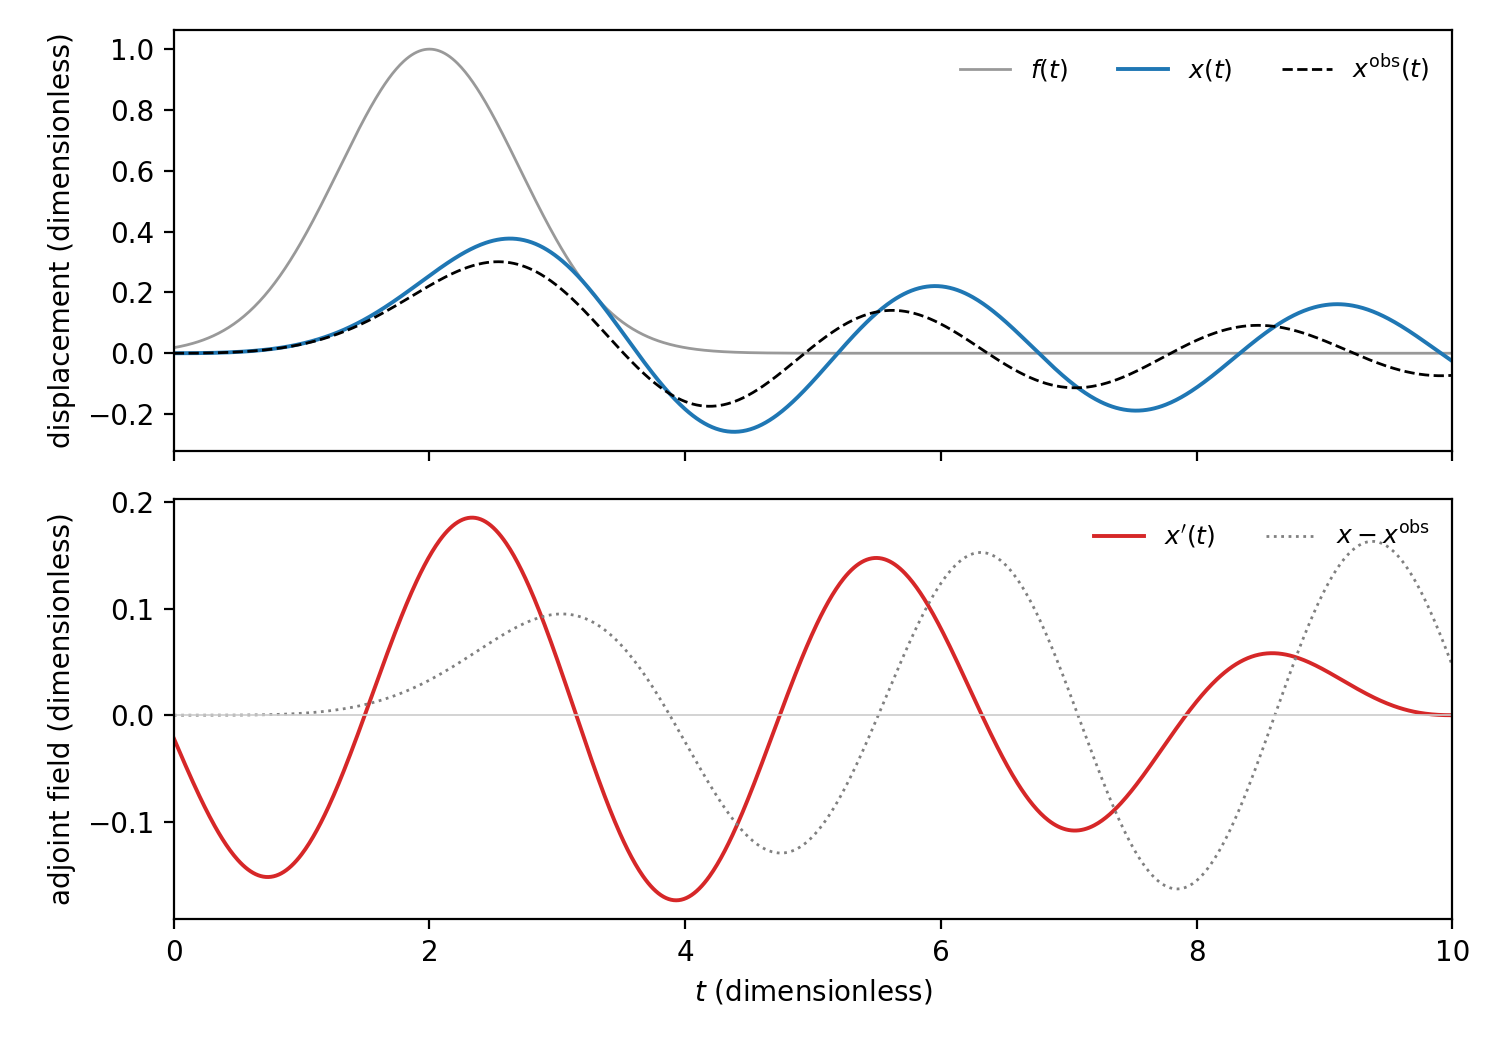
\includegraphics[width=0.7\textwidth]{figures_ex/ex8_oscillator.png}
    \caption{Upper panel: the forcing $f$, the synthetic $x$ for $\omega_{0}=2$, $\gamma=0.1$, and the ``observed'' record
    $x^{\mathrm{obs}}$ generated with $\omega_{0}=2.2$, $\gamma=0.15$. Lower panel: the adjoint field $x'$ obtained by
    integrating eq.~(\ref{eq:15}) backwards from $t=T=10$, together with the residual that drives it. The adjoint field vanishes,
    with zero slope, at $t=T$ and is largest at early times.}
    \label{fig:1}
\end{figure}

\emph{Numerical check.} The forward equation, the adjoint equation (backwards from $t=T$) and the two integrals in
eq.~(\ref{eq:17}) were computed with an eighth-order Runge--Kutta integrator at relative tolerance $10^{-12}$; the fields are
shown in Fig.~\ref{fig:1}. The misfit is $J=4.09742\times10^{-2}$ and the adjoint formulae give
\begin{equation}
\frac{\partial J}{\partial\omega_{0}^{2}}=-0.107897,\qquad \frac{\partial J}{\partial\gamma}=-0.316192.
\label{eq:18}
\end{equation}
Central differences of $J$ with step $h=10^{-4}$ in each parameter give $-0.107897$ and $-0.316192$ respectively, the relative
differences from eq.~(\ref{eq:18}) being $9\times10^{-11}$ and $3\times10^{-7}$; with $h=10^{-3}$ the finite-difference value
for $\gamma$ moves to $-0.316201$, a change consistent with the $O(h^{2})$ truncation error of the difference formula. Both
derivatives are negative, as they should be: the observed record was made with larger $\omega_{0}$ and $\gamma$, and so
increasing either parameter reduces the misfit. For the source kernel, taking $\delta f=\epsilon\sin3t$ gives
$\int_{0}^{T}x'\sin3t\dd t=-1.68008\times10^{-2}$ by the adjoint formula, against a finite-difference value of
$-1.68008\times10^{-2}$. Two integrations of a second-order equation have thus produced the derivatives with respect to every parameter, including the whole function $f$.
\end{solution}

%-----------------------------------------------------------------------------------------------
\begin{example}{Steepest descent on a quadratic misfit}
Let $J(\mathbf{m})=\frac{1}{2}\mathbf{m}^{T}\mathbf{H}\mathbf{m}-\mathbf{b}^{T}\mathbf{m}$ with $\mathbf{H}$ symmetric and positive
definite, and let $\mathbf{g}=\mathbf{H}\mathbf{m}-\mathbf{b}$ be its gradient. Show that the step length minimising
$f(\lambda)=J(\mathbf{m}-\lambda\mathbf{g})$ is $\lambda=\mathbf{g}^{T}\mathbf{g}/\mathbf{g}^{T}\mathbf{H}\mathbf{g}$.
Writing $\mathbf{e}=\mathbf{m}-\overline{\mathbf{m}}$ for the error relative to the minimiser and
$\|\mathbf{e}\|_{\mathbf{H}}^{2}=\mathbf{e}^{T}\mathbf{H}\mathbf{e}$, show that one steepest-descent step satisfies
$\|\mathbf{e}_{1}\|_{\mathbf{H}}^{2}\le\left(\frac{\kappa-1}{\kappa+1}\right)^{2}\|\mathbf{e}_{0}\|_{\mathbf{H}}^{2}$,
where $\kappa$ is the condition number of $\mathbf{H}$. Illustrate with $\mathbf{H}=\mathrm{diag}(1,9)$, $\mathbf{b}=\mathbf{0}$,
starting from $\mathbf{m}_{0}=(9,1)^{T}$.
\end{example}

\begin{solution}
Near a minimum any smooth misfit is approximately quadratic, with $\mathbf{H}$ the Hessian, so this example describes the
asymptotic behaviour of the method of steepest descent described in the lecture. Since $\mathbf{H}$ is positive definite the
unique minimiser is $\overline{\mathbf{m}}=\mathbf{H}^{-1}\mathbf{b}$, and expanding about it,
\begin{equation}
J(\mathbf{m})=J(\overline{\mathbf{m}})+\mathbf{e}^{T}(\mathbf{H}\overline{\mathbf{m}}-\mathbf{b})+\frac{1}{2}\mathbf{e}^{T}\mathbf{H}\mathbf{e}
=J(\overline{\mathbf{m}})+\frac{1}{2}\|\mathbf{e}\|_{\mathbf{H}}^{2},
\label{eq:19}
\end{equation}
so that the $\mathbf{H}$-norm of the error measures the excess misfit, and $\mathbf{g}=\mathbf{H}\mathbf{e}$.

\emph{Step length.} Along the search direction,
\begin{equation}
f(\lambda)=J(\mathbf{m}-\lambda\mathbf{g})=J(\mathbf{m})-\lambda\,\mathbf{g}^{T}\mathbf{g}+\frac{\lambda^{2}}{2}\mathbf{g}^{T}\mathbf{H}\mathbf{g},
\label{eq:20}
\end{equation}
a convex quadratic in $\lambda$, and $f'(\lambda)=0$ gives
\begin{equation}
\lambda=\frac{\mathbf{g}^{T}\mathbf{g}}{\mathbf{g}^{T}\mathbf{H}\mathbf{g}}.
\label{eq:21}
\end{equation}
This is the one-dimensional minimisation referred to in the lecture, here solvable in closed form. For a general misfit the
same expression is obtained by fitting a parabola to $f(0)$, $f'(0)=-\|\mathbf{g}\|^{2}$ and one trial value $f(\lambda_{\mathrm{t}})$,
which costs one extra forward calculation.

\emph{Contraction.} With $\mathbf{e}_{1}=\mathbf{e}_{0}-\lambda\mathbf{g}$ and $\mathbf{g}=\mathbf{H}\mathbf{e}_{0}$,
\begin{equation}
\|\mathbf{e}_{1}\|_{\mathbf{H}}^{2}=\mathbf{e}_{0}^{T}\mathbf{H}\mathbf{e}_{0}-2\lambda\,\mathbf{g}^{T}\mathbf{H}\mathbf{e}_{0}+\lambda^{2}\mathbf{g}^{T}\mathbf{H}\mathbf{g}
=\|\mathbf{e}_{0}\|_{\mathbf{H}}^{2}-\frac{(\mathbf{g}^{T}\mathbf{g})^{2}}{\mathbf{g}^{T}\mathbf{H}\mathbf{g}},
\label{eq:22}
\end{equation}
where we used $\mathbf{g}^{T}\mathbf{H}\mathbf{e}_{0}=\mathbf{g}^{T}\mathbf{g}$ and eq.~(\ref{eq:21}). Since also
$\|\mathbf{e}_{0}\|_{\mathbf{H}}^{2}=\mathbf{g}^{T}\mathbf{H}^{-1}\mathbf{g}$,
\begin{equation}
\frac{\|\mathbf{e}_{1}\|_{\mathbf{H}}^{2}}{\|\mathbf{e}_{0}\|_{\mathbf{H}}^{2}}
=1-\frac{(\mathbf{g}^{T}\mathbf{g})^{2}}{(\mathbf{g}^{T}\mathbf{H}\mathbf{g})(\mathbf{g}^{T}\mathbf{H}^{-1}\mathbf{g})}.
\label{eq:23}
\end{equation}
It remains to bound the second term from below, which is the content of the Kantorovich inequality. Let
$0<\mu_{1}\le\dots\le\mu_{n}$ be the eigenvalues of $\mathbf{H}$, with orthonormal eigenvectors $\mathbf{v}_{i}$, and without
loss of generality take $\|\mathbf{g}\|=1$. Setting $c_{i}=(\mathbf{g}\cdot\mathbf{v}_{i})^{2}$, so that $c_{i}\ge0$ and
$\sum_{i}c_{i}=1$, we have $a\equiv\mathbf{g}^{T}\mathbf{H}\mathbf{g}=\sum_{i}c_{i}\mu_{i}$ and
$b\equiv\mathbf{g}^{T}\mathbf{H}^{-1}\mathbf{g}=\sum_{i}c_{i}/\mu_{i}$. For any $\mu\in[\mu_{1},\mu_{n}]$ we have
$(\mu-\mu_{1})(\mu_{n}-\mu)\ge0$, which on dividing by $\mu$ reads $\mu+\mu_{1}\mu_{n}/\mu\le\mu_{1}+\mu_{n}$. Applying this
to each eigenvalue and summing with weights $c_{i}$ gives $a+\mu_{1}\mu_{n}b\le\mu_{1}+\mu_{n}$, and then by the
arithmetic--geometric mean inequality
\begin{equation}
2\sqrt{\mu_{1}\mu_{n}\,ab}\le a+\mu_{1}\mu_{n}b\le\mu_{1}+\mu_{n}
\quad\Longrightarrow\quad
ab\le\frac{(\mu_{1}+\mu_{n})^{2}}{4\mu_{1}\mu_{n}}.
\label{eq:24}
\end{equation}
Inserting this into eq.~(\ref{eq:23}), and writing $\kappa=\mu_{n}/\mu_{1}$,
\begin{equation}
\frac{\|\mathbf{e}_{1}\|_{\mathbf{H}}^{2}}{\|\mathbf{e}_{0}\|_{\mathbf{H}}^{2}}\le1-\frac{4\mu_{1}\mu_{n}}{(\mu_{1}+\mu_{n})^{2}}
=\left(\frac{\mu_{n}-\mu_{1}}{\mu_{n}+\mu_{1}}\right)^{2}=\left(\frac{\kappa-1}{\kappa+1}\right)^{2}.
\label{eq:25}
\end{equation}
Equivalently the $\mathbf{H}$-norm of the error, and hence the square root of the excess misfit, contracts by at least the
factor $(\kappa-1)/(\kappa+1)$ per iteration. The bound is attained when $\mathbf{g}$ has equal weight on the extreme
eigenvectors and none elsewhere, and the iteration never escapes this situation, as the example below shows.

\begin{figure}[ht]
    \centering
    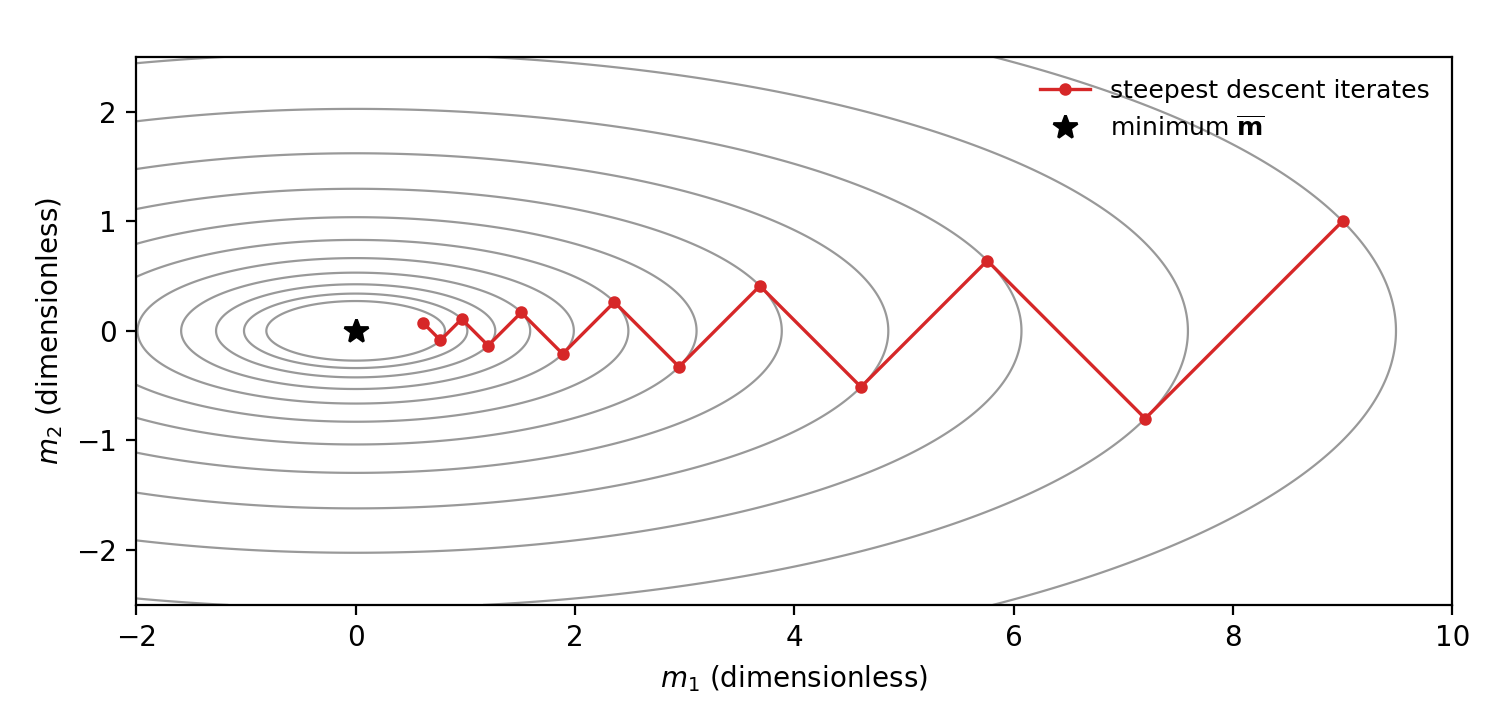
\includegraphics[width=0.7\textwidth]{figures_ex/ex8_steepest.png}
    \caption{Steepest descent with exact line search on $J=\frac{1}{2}(m_{1}^{2}+9m_{2}^{2})$ from $\mathbf{m}_{0}=(9,1)^{T}$.
    Contours are drawn at the misfit values $J_{k}=45\times0.64^{k}$ attained by the iterates, which zigzag between the two
    lines $m_{2}=\pm m_{1}/9$.}
    \label{fig:2}
\end{figure}

\emph{The $2\times2$ example.} For $\mathbf{H}=\mathrm{diag}(1,9)$ we have $\kappa=9$ and
$[(\kappa-1)/(\kappa+1)]^{2}=0.64$. With $\mathbf{b}=\mathbf{0}$ the minimiser is the origin and $\mathbf{e}=\mathbf{m}$.
From $\mathbf{m}_{0}=(9,1)^{T}$ the gradient is $\mathbf{g}_{0}=(9,9)^{T}$, so
$\lambda=162/(81+729)=\frac{1}{5}$ and $\mathbf{m}_{1}=(9,1)^{T}-\frac{1}{5}(9,9)^{T}=\frac{4}{5}(9,-1)^{T}$. The new
gradient $\frac{4}{5}(9,-9)^{T}$ again has components of equal magnitude, so the step length is again $\frac{1}{5}$, and by
induction
\begin{equation}
\mathbf{m}_{k}=\left(\frac{4}{5}\right)^{k}\begin{pmatrix}9\\(-1)^{k}\end{pmatrix},\qquad
J(\mathbf{m}_{k})=45\times\left(\frac{16}{25}\right)^{k}.
\label{eq:26}
\end{equation}
The misfit falls by exactly the factor $0.64$ predicted by eq.~(\ref{eq:25}) at every step, and the iterates zigzag
across the valley as shown in Fig.~\ref{fig:2}. To reduce the misfit by a factor of $10^{6}$ requires
$6/\log_{10}(1/0.64)=31.0$, i.e.\ $31$ iterations ($J_{31}/J_{0}=0.64^{31}=9.8\times10^{-7}$). For $\kappa=100$ the
factor is $(99/101)^{2}=0.9608$ and the same reduction needs $346$ iterations, while for $\kappa=10^{4}$ it would need
about $3.5\times10^{4}$. By contrast, a start on an eigenvector, such as $\mathbf{m}_{0}=(0,3)^{T}$, reaches the minimum in
one step. This slow, zigzagging convergence for ill-conditioned problems is why practical waveform inversions use
conjugate-gradient or quasi-Newton directions built from the history of gradients, as remarked in the lecture; each iteration
still costs the same adjoint calculation, but far fewer of them are needed.
\end{solution}

%-----------------------------------------------------------------------------------------------
\begin{example}{The adjoint traction for a cross-correlation delay time}
Let $s(t)=w(t)\hat{\nu}_{i}u_{i}(\mathbf{x}_{r},t)$ be a windowed component of the synthetic seismogram and
$s^{\mathrm{obs}}(t)$ the corresponding observed quantity, and let $\overline{\tau}$ be defined by
$\dot{C}(\overline{\tau})=0$, where $C(\tau)=\int_{-\infty}^{\infty}s^{\mathrm{obs}}(t-\tau)s(t)\dd t$ and the maximum of
$C$ is meant. By implicit differentiation find the first-order change $\delta\overline{\tau}$ produced by a perturbation
$\delta s(t)$ of the synthetic, and hence the adjoint traction $h_{i}'$ appropriate to the misfit $\overline{\tau}$. Simplify
the result under the assumption that the observed and synthetic waveforms have the same shape, and verify the formulae
numerically on a pair of pulses.
\end{example}

\begin{solution}
The lecture noted that the whole adjoint apparatus carries over to any misfit once the corresponding adjoint traction is known,
since the form of $J$ enters only through $h_{i}'$. Here the ``misfit'' is the delay time itself, and its functional derivative
with respect to the wavefield is what we need.

\emph{Sign convention.} It is worth being clear about what $\overline{\tau}$ measures. If the observed waveform is a delayed
copy of the synthetic, $s^{\mathrm{obs}}(t)=s(t-\Delta)$, then $C(\tau)=\int s(t-\Delta-\tau)s(t)\dd t$ is maximised when
$\tau=-\Delta$. Thus with the definition used in the lecture, $\overline{\tau}$ is positive when the synthetic arrives
\emph{later} than the observation; it is the negative of the delay time as usually quoted. Some authors define the
cross-correlation with $s^{\mathrm{obs}}(t+\tau)$ or with $s(t-\tau)$ so as to reverse this, and all that changes below is the
overall sign of $h_{i}'$.

\emph{Implicit differentiation.} Differentiating under the integral sign, and using
$\partial_{\tau}s^{\mathrm{obs}}(t-\tau)=-\dot{s}^{\mathrm{obs}}(t-\tau)$,
\begin{equation}
\dot{C}(\tau)=-\int_{-\infty}^{\infty}\dot{s}^{\mathrm{obs}}(t-\tau)s(t)\dd t=\int_{-\infty}^{\infty}s^{\mathrm{obs}}(t-\tau)\dot{s}(t)\dd t,
\label{eq:27}
\end{equation}
the second form following by an integration by parts in which the boundary terms vanish because the window $w$ confines $s$
to a finite interval. The defining condition $F(\overline{\tau},s)\equiv\dot{C}(\overline{\tau})=0$ makes $\overline{\tau}$ an
implicit function of $s$. Perturbing $s\to s+\delta s$ and $\overline{\tau}\to\overline{\tau}+\delta\overline{\tau}$ in the
second form of eq.~(\ref{eq:27}) and expanding to first order,
\begin{equation}
\underbrace{\int s^{\mathrm{obs}}(t-\overline{\tau})\dot{s}(t)\dd t}_{=0}
-\delta\overline{\tau}\int\dot{s}^{\mathrm{obs}}(t-\overline{\tau})\dot{s}(t)\dd t
+\int s^{\mathrm{obs}}(t-\overline{\tau})\delta\dot{s}(t)\dd t=0.
\label{eq:28}
\end{equation}
The coefficient of $\delta\overline{\tau}$ is $\ddot{C}(\overline{\tau})$, which is negative at a maximum, and the last integral can be
integrated by parts. Hence
\begin{equation}
\delta\overline{\tau}=\frac{1}{\ddot{C}(\overline{\tau})}\int_{-\infty}^{\infty}\dot{s}^{\mathrm{obs}}(t-\overline{\tau})\,\delta s(t)\dd t,
\label{eq:29}
\end{equation}
where
\begin{equation}
\ddot{C}(\overline{\tau})=-\int_{-\infty}^{\infty}\dot{s}^{\mathrm{obs}}(t-\overline{\tau})\dot{s}(t)\dd t
=\int_{-\infty}^{\infty}s^{\mathrm{obs}}(t-\overline{\tau})\ddot{s}(t)\dd t.
\label{eq:30}
\end{equation}
This is exact, and involves only quantities available after the forward calculation: the shifted observed waveform and the
synthetic. A useful check is a perturbation that simply delays the synthetic by $\epsilon$, $\delta s=-\epsilon\dot{s}$; then
eq.~(\ref{eq:29}) gives $\delta\overline{\tau}=+\epsilon$ exactly, as the sign convention above requires, and this holds
whatever the shape of $s^{\mathrm{obs}}$.

\emph{The equal-shape approximation.} The measured $\overline{\tau}$ is the shift that best aligns the two waveforms, and if
they have the same shape, $s^{\mathrm{obs}}(t-\overline{\tau})\approx s(t)$, which in the lecture's convention is the
statement $s^{\mathrm{obs}}(t)\approx s(t+\overline{\tau})$. (The form $s^{\mathrm{obs}}(t)\approx s(t-\overline{\tau})$ often written
corresponds to the opposite sign convention for $\tau$.) Under this assumption eq.~(\ref{eq:29}) becomes
\begin{equation}
\delta\overline{\tau}\approx-\frac{\displaystyle\int_{-\infty}^{\infty}\dot{s}(t)\,\delta s(t)\dd t}{\displaystyle\int_{-\infty}^{\infty}\dot{s}(t)^{2}\dd t},
\label{eq:31}
\end{equation}
where the denominator, $\ddot{C}(\overline{\tau})\approx\int s\ddot{s}\dd t=-\int\dot{s}^{2}\dd t$, is manifestly negative.
The observed data have disappeared entirely from the linearised relation: they enter only through the value of
$\overline{\tau}$. An overall amplitude difference between $s^{\mathrm{obs}}$ and $s$ also drops out, since it cancels between the
numerator and denominator of eq.~(\ref{eq:29}), so the approximation is really one of equal shape rather than equal waveform.

\emph{Adjoint traction.} The window and the component $\hat{\bm{\nu}}$ are fixed, so that a change in the wavefield
produces $\delta s(t)=w(t)\hat{\nu}_{i}\delta u_{i}(\mathbf{x}_{r},t)$, and the integrals may be restricted to $[0,T]$.
Comparing with the form
$\langle DJ(\mathbf{u})|\delta\mathbf{u}\rangle=\int_{0}^{T}\int_{\partial M}h_{i}'\,\delta u_{i}\dd S\dd t$ used in the
lecture, we read off
\begin{align}
h_{i}'(\mathbf{x},t)&=\frac{w(t)\,\dot{s}^{\mathrm{obs}}(t-\overline{\tau})}{\ddot{C}(\overline{\tau})}\,\hat{\nu}_{i}\,\delta(\mathbf{x}-\mathbf{x}_{r}) \nonumber \\
&\approx-\frac{w(t)\,\dot{s}(t)}{\int_{0}^{T}\dot{s}^{2}\dd t}\,\hat{\nu}_{i}\,\delta(\mathbf{x}-\mathbf{x}_{r}).
\label{eq:32}
\end{align}
The adjoint traction is therefore, up to a normalising constant, the time derivative of the windowed synthetic, applied at the
receiver in the direction of the measured component. Everything else in the lecture goes through unchanged: $\mathbf{u}'$
solves the adjoint wave equation with terminal conditions and this traction, and $\delta\overline{\tau}$ follows from the
kernels $K_{\rho}$ and $K_{A_{ijkl}}$. For an isotropic model,
$\delta A_{ijkl}=(\delta\kappa-\frac{2}{3}\delta\mu)\delta_{ij}\delta_{kl}+\delta\mu(\delta_{ik}\delta_{jl}+\delta_{il}\delta_{jk})$,
and with $\rho$ held fixed $\delta\mu=2\rho\beta\,\delta\beta$ and $\delta\kappa=2\rho\alpha\,\delta\alpha-\frac{8}{3}\rho\beta\,\delta\beta$,
which is how the kernels $K_{\alpha}$ and $K_{\beta}$ of the lecture are assembled from $K_{A_{ijkl}}$. Because $h_{i}'$ is
proportional to $\dot{s}$ rather than to a residual, the kernel does not vanish when the data are fit perfectly; it is the
sensitivity of a measurement, not of a misfit, and this is what gives the banana--doughnut kernels their universal form.

\emph{Numerical check.} Take $s(t)=(t-t_{0})\ee^{-(t-t_{0})^{2}/\sigma^{2}}$ with $t_{0}=5$, $\sigma=0.6$, and observed pulses
$s^{\mathrm{obs}}(t)=a\,(t-t_{0}-\Delta)\ee^{-(t-t_{0}-\Delta)^{2}/\sigma_{\mathrm{obs}}^{2}}$ with $\Delta=0.4$, the record
$[0,12]$ containing both pulses entirely. In every case below the root of $\dot{C}$ is $\overline{\tau}=-0.4000$, confirming
the sign convention; because both pulses are antisymmetric about their centres, $C$ is symmetric about $\tau=-\Delta$ and the
result is exact even when the shapes differ. We then perturb $s\to s+\epsilon\,\eta$ with
$\eta(t)=\cos2t\,\ee^{-(t-t_{0}-0.5)^{2}}$, recompute $\overline{\tau}(\pm\epsilon)$ by root finding with $\epsilon=10^{-4}$, and
compare the central difference with eqs.~(\ref{eq:29}) and (\ref{eq:31}) evaluated with $\delta s=\eta$. For identical
shapes ($a=1$, $\sigma_{\mathrm{obs}}=\sigma$) all three agree: $\ddns\overline{\tau}/\ddns\epsilon=0.682928$. For $a=1.2$ and
$\sigma_{\mathrm{obs}}=\sigma$ the numbers are unchanged, as predicted. For $a=1.2$ and $\sigma_{\mathrm{obs}}=1.1\sigma$ the
finite difference gives $0.747030$, the exact formula eq.~(\ref{eq:29}) gives $0.747030$, and the approximate formula
eq.~(\ref{eq:31}) gives $0.682928$, which is $8.6$ per cent low; the discrepancy is entirely in the denominator, with
$\ddot{C}(\overline{\tau})=-0.7018$ against $-\int\dot{s}^{2}\dd t=-0.5640$. For a $2$ per cent width mismatch the error of
eq.~(\ref{eq:31}) is $1.8$ per cent. The equal-shape approximation is thus accurate when it should be, and in practice it is
adopted because it makes the adjoint source independent of the data and hence the kernels a property of the reference model
alone.
\end{solution}

%-----------------------------------------------------------------------------------------------
\begin{example}{Counting the cost}
A tomographic inversion uses $n_{\mathrm{ev}}$ earthquakes, performs $n_{\mathrm{it}}$ iterations of gradient descent, and
each numerical solution of the wave equation costs a time $c$. Estimate the total computational cost of the inversion using
(a) the adjoint method with two or three simulations per event and iteration, and (b) a finite-difference gradient with $m$
model parameters. Put in the numbers from the lecture: $c\approx10$ minutes, $n_{\mathrm{ev}}=10^{2}$--$10^{3}$,
$n_{\mathrm{it}}\approx15$, $m=10^{4}$--$10^{6}$. Explain why three simulations rather than two are usually performed.
\end{example}

\begin{solution}
The misfit is a sum over events, $J=\sum_{e}J_{e}$, and each $J_{e}$ requires its own forward simulation because the source
differs. The gradient is likewise a sum, $DJ=\sum_{e}DJ_{e}$, with each term requiring its own adjoint simulation, since the
adjoint traction $h_{i}'$ is built from that event's residuals.

\emph{Adjoint method.} Per event and iteration we need one forward simulation, to obtain $J_{e}$ and $h_{i}'$, and one
adjoint simulation, to obtain $\mathbf{u}'$ and hence the kernels. The total cost is
\begin{equation}
\mathcal{C}_{\mathrm{adj}}\approx2\,n_{\mathrm{ev}}\,n_{\mathrm{it}}\,c,
\label{eq:33}
\end{equation}
or $3\,n_{\mathrm{ev}}n_{\mathrm{it}}c$ with re-simulation (below). The line search for the step length $\lambda$ adds at
least one further forward simulation per event, so that $3$--$4$ simulations per event and iteration is a realistic count.
Crucially, none of this depends on $m$: the kernels $K_{\rho}$, $K_{A_{ijkl}}$ and $K_{\overline{S}_{ij}}$ are fields,
obtained on the numerical grid at the cost of a few multiplications per grid point and time step, and any parameterisation of
the model can then be projected out of them.

\emph{Finite differences.} The one-sided formula in the lecture requires $J(\mathbf{m})$ and $J(\mathbf{m}+\delta\mathbf{m}_{k})$
for each of the $m$ basis directions, each evaluation being a sum over events. Thus
\begin{equation}
\mathcal{C}_{\mathrm{fd}}\approx(m+1)\,n_{\mathrm{ev}}\,n_{\mathrm{it}}\,c,
\label{eq:34}
\end{equation}
and central differences would double this. The ratio $\mathcal{C}_{\mathrm{adj}}/\mathcal{C}_{\mathrm{fd}}=3/(m+1)$ is the
factor quoted in the lecture.

\emph{Numbers.} Take $n_{\mathrm{ev}}=10^{3}$, $n_{\mathrm{it}}=15$ and $c=10\,\mathrm{min}$. The adjoint method with two
simulations needs $3\times10^{4}$ simulations, or $3\times10^{5}\,\mathrm{min}=5000\,\mathrm{h}\approx208\,\mathrm{days}$
of cluster time; with three simulations this rises to $312\,\mathrm{days}$, and with a trial step for the line search to
about $420\,\mathrm{days}$. With $n_{\mathrm{ev}}=10^{2}$ divide by ten. These are totals of machine time: different events
are independent, so with a hundred simulations running concurrently the wall-clock time for the inversion is a few days,
which is the scale on which the global models shown in the lecture were produced. Finite differences with $m=10^{4}$ need
$1.5\times10^{9}\,\mathrm{min}\approx2.9\times10^{3}$ years, and with $m=10^{6}$ about $2.9\times10^{5}$ years, regardless
of how the work is distributed. There is no parameterisation coarse enough to rescue the finite-difference approach while
retaining anything like the resolution of the grid on which the wave equation is solved.

\emph{Why three simulations.} The kernels in the lecture are time integrals of products of the forward and adjoint fields,
$K_{\rho}=\int_{0}^{T}\partial_{t}u_{i}\,\partial_{t}u_{i}'\dd t$ and so on. The adjoint field is obtained by integrating
backwards from $t=T$, and so at the time step when $\mathbf{u}'(\mathbf{x},t)$ is available, $\mathbf{u}(\mathbf{x},t)$ was
computed long before. Storing the forward field at every time step is impractical: for a global simulation with of order
$10^{9}$ grid points, $10^{4}$ time steps and three components in single precision this is of order
$10^{14}$ bytes per event. Instead one stores only the final state $\mathbf{u}(\mathbf{x},T)$, $\partial_{t}\mathbf{u}(\mathbf{x},T)$
(together with the wavefield on any absorbing boundaries), and during the adjoint calculation integrates the forward
equations \emph{backwards} from this final state alongside the adjoint equations; the elastic wave equation without
attenuation is time-reversible, so this reconstructs $\mathbf{u}$ at each step as it is needed. The kernels are then
accumulated on the fly. The price is a third simulation, and the factor of $3/(m+1)$ in the lecture is the honest
accounting for it.
\end{solution}

\end{document}
